
\item A composite block is made of slabs A, B, C, D and E of different thermal conductivities (given in terms of a constant K) and sizes (given in terms of length, L) as shown in the figure. All slabs are of same width. Heat `Q' flows only from left to right through the blocks. Then in steady state
    \begin{center}
        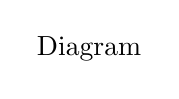
\begin{tikzpicture}
            \node at (0, 0) {Diagram}; % Replace this with the actual TiKZ code for the diagram
        \end{tikzpicture}
    \end{center}
    \begin{tasks}(2)
        \task heat flow through A and E slabs are same.
        \task heat flow through slab E is maximum.
        \task temperature difference across slab E is smallest.
        \task heat flow through C = heat flow through B + heat flow through D.
    \end{tasks}
